%--------------------
% Packages
% -------------------
\documentclass[11pt,a4paper]{article}
\usepackage[utf8x]{inputenc}
\usepackage[T1]{fontenc}


\usepackage[pdftex]{graphicx} % Required for including pictures
\usepackage[english]{babel} % Translations
\usepackage[pdftex,linkcolor=black,pdfborder={0 0 0}]{hyperref} % Format links for pdf
\usepackage{calc} % To reset the counter in the document after title page
\usepackage{enumitem} % Includes lists

%-----------------------
% Begin document
%-----------------------
\begin{document}

\begin{figure}
    \centering
    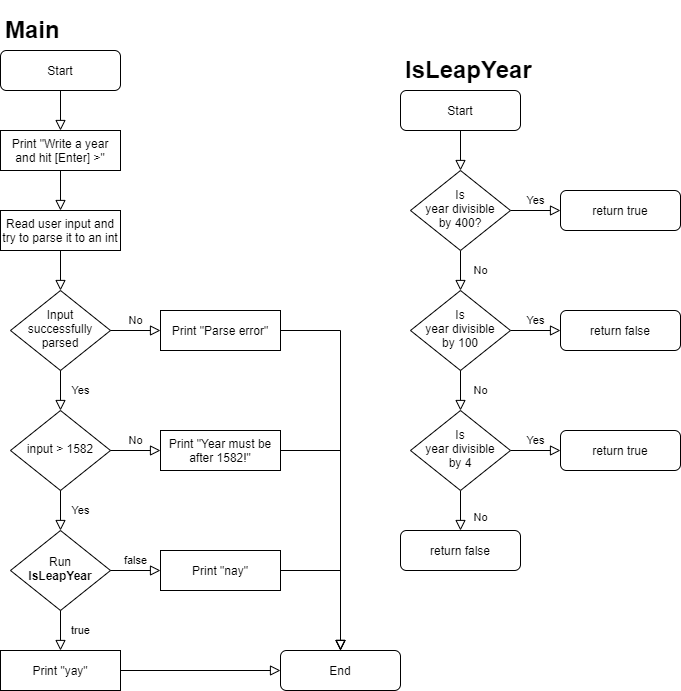
\includegraphics[width=\textwidth]{Documentation/img/IsLeapYear.drawio.png}
    \label{fig:my_label}
\end{figure}

\textbf{The algorithm works as follows:}

First, \texttt{"Write a year and hit [Enter] >"} is written to the console. Then, the user inputs something and presses [Enter].

We then attempt to parse the input to an \texttt{int}. If this is unsuccessful, we write \texttt{"Parse error"} to the console. Otherwise, we check if the input is more than 1582.
If this is \textit{not} the case, we print \texttt{"Year must be after 1582!"} in the console.

If the input \textit{is} more than 1582, we invoke \textbf{IsLeapYear} with the input as the year.
If the result of \textbf{IsLeapYear} is true, we write \texttt{"yay"} to the console. Otherwise, we write \texttt{"nay"}.

\textbf{IsLeapYear:}

If the year is divisible by 400, we return true. If it is not, we check if it is divisible by 100. If it is, we return false. If it is not, we check if it is divisible by 4. If it is, we return true. Otherwise we return false.

\end{document}
